%************************************************
\chapter{Data clustering}\label{sec: clusters}
%************************************************

\section*{Hierarchical clustering and dendograms}
Hierarchical clustering pairwise groups 
variables according to the minimum distances,
and so on and so forth until the entire data 
set is reconstructed and tree shaped. Distances
between points can be calculated using any
distance $d(x,y)$ via
\texttt{dist(df, method = <method>)}, the data frame
containing the rows as points whose distances one
wants to calculate. 
\medskip 

As an example we can hierarchically cluster a subset
of the \texttt{mtcars} data starting from calculating 
its euclidean distances among different rows (which, 
in turn, represent the different points that we want
to cluster)
\begin{verbatim}
distances <- dist(iris, method = "euclidean")
dendog    <- hclust(distances, method = "ave") 
\end{verbatim}
The function \texttt{hclust} pairwise couples the points
according to the minimum distance, going up in pairs until
the whole data set is exhausted.
\bigskip
The dendogram can be plotted making use of the 
following packages:\\
\texttt{library("ggplot2")}\\
\texttt{install.packages("ggdendro")}\\
\texttt{library("ggdendro")}
\bigskip 

\begin{verbatim}
# dendro_data extracts the dendogram 
# objects numerical data
dendog    <- dendro_data(dendog, type = "rectangle")

p <- ggplot(segment(dendog)) 
p <- p + theme(panel.grid.major = element_blank(), 
               panel.grid.minor = element_blank(),
               panel.background = element_rect(fill 
                                               = '#002b36'),
               axis.line = element_line(colour = "black"),
               legend.text=element_text(size=16),
               legend.title=element_blank(),
               axis.title.x = element_text(vjust=0, size=16),
               axis.title.y = element_text(vjust=1, size=16),
               plot.title   = element_text(vjust=1.5, size=20))
p <- p + geom_segment(aes(x = x, y = y, 
                      xend = xend, yend = yend),
                      colour = "white", alpha = 0.7)
p <- p + geom_text(data = label(dendog), colour = "white", 
                   aes(x = x+0.5, y = -5, label = label),
                   vjust = 1.2, hjust = 0)
p <- p + coord_flip()
p <- p + scale_y_reverse(expand = c(0.2, 0))
p <- p + labs(x = "cars")
p <- p + labs(y = "")
show(p)
\end{verbatim}
\begin{figure}[htbp]
 \centering
 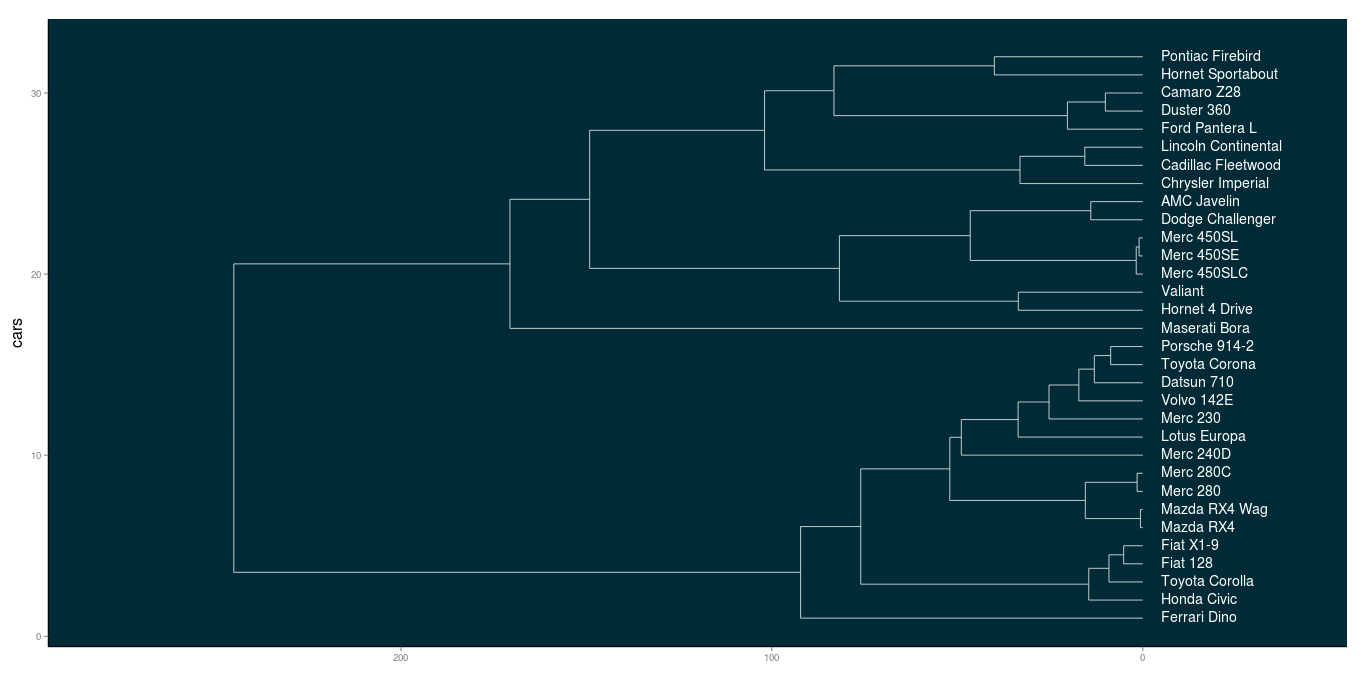
\includegraphics[scale=0.25]{images/dendo}
 \caption*{Hierarchical clustering dendogram}
\end{figure}

\section{$k$-means clustering}
$k$-means clustering groups the data
in clusters according to the shortest
distances to the centres of the cluster,
whose number may be manually set. How to
properly calculate the correct number
of clusters and their centres will not 
be investigated here and we refer the 
reader to standard literature for that.
\bigskip

\texttt{kmeans} needs a set of data whose 
rows represent different point, whose 
coordinates are in turn given as column
entries; all the provided values must be
in numerical format. Different methods to calculate
the clusters can be specified as additional
arguments and options parameters.
\begin{verbatim}
# storing the names 
names <- iris[,5]
iris  <- iris[-5]

cluster <- kmeans(iris, centers = 3)

# coordinates of the centres
R: cluster$centers

  Sepal.Length Sepal.Width Petal.Length Petal.Width
1     5.006000    3.428000     1.462000    0.246000
2     5.901613    2.748387     4.393548    1.433871
3     6.850000    3.073684     5.742105    2.071053

# dimensions of the clusters
R: cluster$size

[1] 50 62 38

# each labelled row belongs to the specified cluster
R: cluster$cluster

  [1] 1 1 1 1 1 1 1 1 1 1 1 1 1 1 1 1 1 1 1 1...
 [38] 1 1 1 1 1 1 1 1 1 1 1 1 1 2 2 3 2 2 2 2...
 [75] 2 2 2 3 2 2 2 2 2 2 2 2 2 2 2 2 2 2 2 2...
[112] 3 3 2 2 3 3 3 3 2 3 2 3 2 3 3 2 2 3 3 3...
[149] 3 2
\end{verbatim}
Additional information can be gained investigating
the outcome values of the function \texttt{kmeans}.
However, row names can be placed back against the 
clusters labels as
\begin{verbatim}
R: table(names, cluster$cluster)
            
names         1  2  3
  setosa     50  0  0
  versicolor  0 48  2
  virginica   0 14 36
\end{verbatim}
\medskip 

Clustering can be made use of to spot 
possible outliers in the set of data, 
as those point having the furthest distances
from any of the clusters centres.
\begin{verbatim}
centres   <- cluster$centers[cluster$cluster,]
distances <- sqrt(rowSums((iris-centres)^2))

outliers  <- head(iris[order(distances, decreasing = TRUE),])

R: outliers

    Sepal.Length Sepal.Width Petal.Length Petal.Width
99           5.1         2.5          3.0         1.1
58           4.9         2.4          3.3         1.0
94           5.0         2.3          3.3         1.0
61           5.0         2.0          3.5         1.0
119          7.7         2.6          6.9         2.3
118          7.7         3.8          6.7         2.2
\end{verbatim}
The above can be made into a function, such that, given 
a data set, one can return the first $M$ outliers once 
a clustering around $N$ groups has been performed:
\begin{verbatim}
outlier.by.clustering <- function(df,N,M){
    cluster   <- kmeans(df, centers = N)
    centres   <- cluster$centers[cluster$cluster,]
    distances <- sqrt(rowSums((df-centres)^2))
    outliers  <- head(df[order(distances, 
                      decreasing = TRUE),],M)
    return(outliers)
}

R: outlier.by.clustering(iris,3,5)

    Sepal.Length Sepal.Width Petal.Length Petal.Width
99           5.1         2.5          3.0         1.1
58           4.9         2.4          3.3         1.0
94           5.0         2.3          3.3         1.0
61           5.0         2.0          3.5         1.0
119          7.7         2.6          6.9         2.3
\end{verbatim}



